\documentclass[a4paper]{article}

%% Language and font encodings
\usepackage{polski}
\usepackage[utf8]{inputenc}
\usepackage[T1]{fontenc}
\usepackage{pdfpages}
\usepackage{indentfirst}
\usepackage{cancel}

% Adjust penalties
\brokenpenalty=1000
\clubpenalty=1000
\widowpenalty=1000

%% Sets page size and margins
\usepackage[a4paper]{geometry}

%% Useful packages
\usepackage{amsmath}
\usepackage{graphicx}
\usepackage[colorlinks=true, allcolors=blue]{hyperref}
\usepackage{booktabs}
\usepackage{ulem}
\usepackage{tikz}

\usepackage{float}

\renewcommand\thesection{\arabic{section}.}
\renewcommand\thesubsection{\arabic{section}.\arabic{subsection}.}
\renewcommand\thesubsubsection{\arabic{section}.\arabic{subsection}. \arabic{subsubsection}.}

% The following commands are not supported in PSTricks at present
% We define them conditionally, so when they are implemented,
% this pgf file will use them.
\ifx\du\undefined
  \newlength{\du}
\fi
\setlength{\du}{15\unitlength}

\newcommand{\Vsp}[1]{\vtop to #1 {}}
\newcommand{\Hsp}[1]{\hbox to #1 {}}
\newcommand{\Small}{\scriptsize}

\title{Sprawozdanie nr 5}
\date{}


\begin{document}

\begin{center}
\begin{tabular}{|p{5.5cm}|l|l|c|}
    \hline
	% Row 1.1  
	    Wydział \Vsp{4mm} &
	    \multicolumn{1}{|l}{Dzień} &
	    poniedziałek $17^{15} - 19^{30}$ &
	    Nr zespołu \\
	% Row 1.2
	    \mbox{\small{Matematyki i Nauk Informatycznych}} &
	    \multicolumn{1}{|l}{Data}  &
	    &
	    \multicolumn{1}{c|}{\Large{18}} \\
    
    \hline
	% Row 2.1 
	    Nazwisko i Imię: &
	    \Small Ocena z przygotowania &
	    \Small Ocena ze sprawozdania &
	    \Small Ocena Końcowa \\
	% Rows 2.2-2.4
	    1. Jasiński Bartosz & & &\\
	    2. Sadłocha Adrian & & & \\
	    3. Wódkiewicz Andrzej & & & \\

    \hline
    % Row 3.1
	    \multicolumn{2}{|l|}{Prowadzący \Vsp{4mm}} &
	    \multicolumn{2}{|l|}{Podpis prowadzącego} \\  
    % Row 3.2
    	\multicolumn{2}{|l|}{} &
    	\multicolumn{2}{|l|}{} \\    	
    \hline
\end{tabular}
\label{pieczatka}
\end{center}

{\let\newpage\relax\maketitle}  % stolen from: https://tex.stackexchange.com/questions/86249/maketitle-text-before-title
\setcounter{secnumdepth}{2}


\section{Opis ćwiczenia}
Ćwiczenie złożone było z następujących części:
\begin{enumerate}
	\item{Badanie prawa Malusa}
	\item{Badanie prawa Snella}
	\item{Wyznaczenie kąta granicznego}
	\item{Wyznaczenie kąta Brewstera}
\end{enumerate}

\subsection{Wstęp teoretyczny}
\subsection{Układ pomiarowy}



\section{Pomiary i obliczenia}
\subsection{Badanie prawa Malusa}
Przy pomocy obu polaryzatorów oraz fotodetektora została zmierzona wartość natężenia światła spolaryzowanego.
Wpierw odnaleziony został taki kąt obrotu analizatora, przy którym mierzona wartość natężenia światła była maksymalna ($\alpha_0 = 176^\circ$).
Następnie, siedmiokrotnie dokonano obrotu analizatora o $15^\circ$ i pomiaru wartości natężenia.
Wyniki zostały przedstawione w tablicy \ref{malus-pomiary}. 
% Pomiary 1. i 7. zostały uznane jako błędy grube na podstawie próby dopasowania wykresu funkcji $263 \cos^2(x+10)$ do wyników pomiarów (patrz rysunek \ref{malus-wykres}).
Na rysunku \ref{malus-wykres} przedstawione zostały 2 próby jak najlepszego dopasowania wykresu funkcji $\cos^2$ uwzględniając wszystkie niepewności standardowe, przy założeniach:
\begin{itemize}
	\item kąt $\alpha_0$ jest kątem, dla którego natężenie jest maksymalne -- kolor czerwony
	\item kąty obrotu analizatora zostały odczytane z przesunięciem $10^\circ$, pomiar $k=1$ jest błędem grubym, a kąt $\alpha_0$ \textbf{nie} jest kątem maksymalnego natężenia -- kolor zielony
\end{itemize}

Biorąc pod uwagę trudności podczas przeprowadzania ćwiczenia, pomimo większej ilości założeń prawdziwy zdaje się być przypadek drugi (kolor zielony na wykresie).


\begin{table}[h]
\centering
\begin{tabular}{rrrr}
\toprule
 $k$ &  $\alpha_k \ ({}^\circ)$ &  $I \ (\mu\text{A})$ &  $u_I \ (\mu \text{A})$ \\
\midrule
 0 &       176 &   260.0 &         3.662877 \\
 \textit{1} & 	   \textit{161} &   \textit{240.0} &         \textit{3.662877} \\
 2 &       146 &   225.0 &         3.662877 \\
 3 &       131 &   160.0 &         3.662877 \\
 4 &       116 &    94.0 &         1.414214 \\
 5 &       101 &    32.0 &         1.414214 \\
 6 &        86 &     2.2 &         0.036629 \\
 7 &        71 &    13.0 &         0.366288 \\
\bottomrule
\end{tabular}
\caption{Pomiary natężenia światła spolaryzowanego}
\label{malus-pomiary}
\end{table}



\begin{figure}[h]
\centering
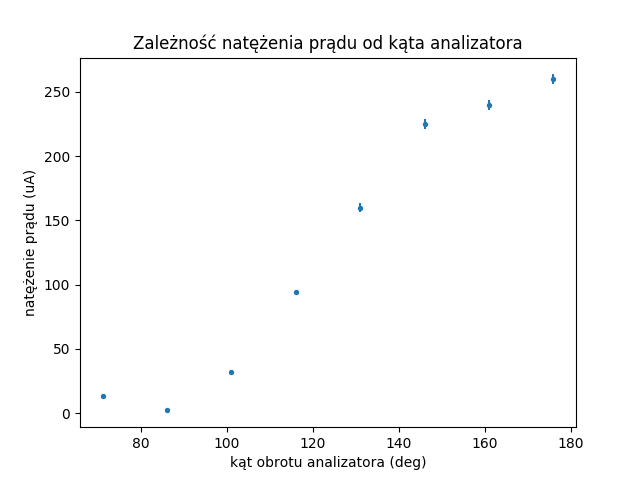
\includegraphics[scale=0.6]{malus.png}
\caption{Prawo Malusa}
\label{malus-wykres}
\end{figure}


\subsection{Badanie prawa Snella}
Następnie, wykonano pomiary prowadzące do wyznaczenia współczynnika załamania światła dla płytki z pleksiglasu.
W tym celu zmierzono kąty padania światła, jak i kąty odbicia.
Wyniki zostały przedstawione w tabeli \ref{snell-pomiary}.
Niepewność pomiaru typu B wyniosła $1.5^\circ$, stąd standardowa niepewność pomiarowa, podana w radianach jest równa $u_x = \frac{1.5 \cdot 2 \pi}{360 \cdot \sqrt{3}} = 0.015115$.
Korzystając z metody propagacji błędu dla pomiarów pośrednich, jakimi są sinusy mierzonych kątów, otrzymujemy, że:
\[
	u_{\sin(x)} = \sqrt{\left(\frac{\partial \sin(x)}{\partial x}u_{x}\right)^2} = \left|\cos(x)u_{x}\right|
\]

Pomiary wraz z niepewnościami na iksach i igrekach zostały naniesione na wykresie (rysunek \ref{snell-wykres}).
Następnie, korzystając z metody najmniejszych kwadratów, zostało odnalezione najlepsze dopasowanie funkcji liniowej, przedstawione na wykresie kolorem czerwonym.
Skorzystano z poniższych wzorów:
\begin{align*}
a &= \frac{n \Sigma X Y - \Sigma X \Sigma Y}{n \Sigma X^2 - \left(\Sigma X\right)^2} \\
b &= \frac{1}{n}\left(\Sigma Y - a \Sigma X\right) \\
u(a) &= \sqrt{\frac{n}{n-2} \frac{\Sigma Y^2 - a\Sigma XY - b\Sigma Y}{n\Sigma X^2-\left(\Sigma X \right)^2}} \\
u(b) &= u(a)\cdot \sqrt{\frac{\Sigma X^2}{n}}
\end{align*}
gdzie $X = \sin\alpha, \ Y = \sin\beta, \ n = 7$.


Współczynnik nachylenia prostej wyniósł $a = 0.66688$, a wyraz wolny: $b = 0.00415$.
Niepewności uzyskanych wartości to odpowiednio:
$ u_a=0.00591, \ u_b=0.00411 $

Zatem, korzystając z prawa Snella:
\begin{align*}
\frac{n_2}{n_1} &= \frac{\sin\alpha}{\sin\beta} \\ 
\frac{n_2}{n_1} &= \frac{\sin\alpha}{a \cdot \sin\alpha + b}
\end{align*}

Zakładając, że $n_1 \approx 1, \ b \approx 0$ otrzymujemy:
\[ n_2 = \frac{1}{a}\]

Stąd: $n_2 = \frac{1}{0.66688} \approx 1.49952$

Niepewność standardową otrzymanego wyniku otrzymamy ponownie ze wzoru na propagację błędu:

\[
		u_{n_2(a)} = \sqrt{\left(\frac{\partial n_2(a)}{\partial a}u_{a}\right)^2} = 
		\left| \frac{1}{a^2} u_{a}\right| = \frac{1}{0.66688^2}\cdot 0.00591 \approx 0.01329
\]

Zatem uwzględniając niepewność standardową, współczynnik załamania światła płytki wykorzystanej w ćwiczeniu (obliczony przy użyciu metody wykorzystującej prawo Snella) wynosi \[ n_2 = 1.500(13)\]
\begin{table}
\centering
\begin{tabular}{lrrrrrrrr}
\toprule

l.p.&  $\alpha \ ({}^\circ)$ & $\beta \ ({}^\circ)$ &  $\alpha \ (\text{rad})$ &  $\beta \ (\text{rad})$ &  $\sin(\alpha)$ &  $\sin(\beta)$ &  $u_{\sin(\alpha)}$ &  $u_{\sin(\beta)}$ \\
\midrule
0  &           5 &         3.5& 0.087266 &    0.061087 &   0.087156 &   0.061049 &              0.015057 &              0.015087 \\
1  &          15 &        10.5 & 0.261799 &    0.183260 &   0.258819 &   0.182236 &              0.014600 &              0.014862 \\
2 & 30 & 19.5 &0.523599 &    0.340339 &   0.500000 &   0.333807 &              0.013090 &              0.014248 \\
3&          45 &        28.0 & 0.785398 &    0.488692 &   0.707107 &   0.469472 &              0.010688 &              0.013346 \\
4&          60 &        36.0 & 1.047198 &    0.628319 &   0.866025 &   0.587785 &              0.007557 &              0.012228 \\
5  &          70 &        39.0& 1.221730 &    0.680678 &   0.939693 &   0.629320 &              0.005170 &              0.011747 \\
6 &          75 &        40.5& 1.308997 &    0.706858 &   0.965926 &   0.649448 &              0.003912 &              0.011494 \\
\bottomrule
\end{tabular}

\caption{Pomiary zależności kąta odbicia ($\beta$) od kąta padania ($\alpha$)}
\label{snell-pomiary}
\end{table}


\begin{figure}[h]
\centering
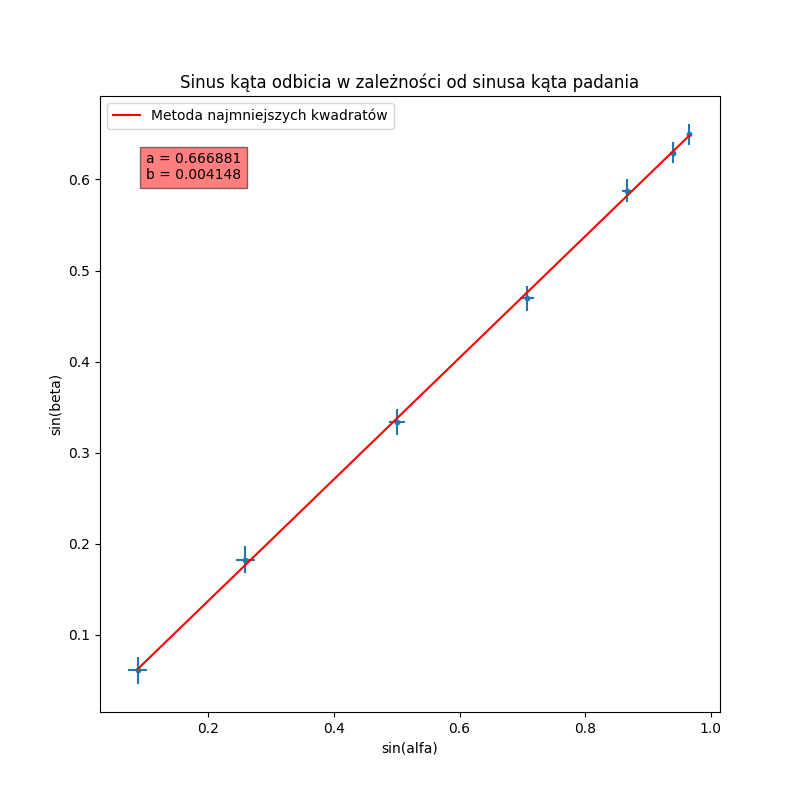
\includegraphics[scale=0.7]{snell.png}
\caption{Prawo Snella}
\label{snell-wykres}
\end{figure}


\subsection{Wyznaczenie kąta granicznego}
\subsection{Wyznaczenie kąta Brewstera}


\subsection{Wnioski}


\end{document}
